%%%%%%%%%%%%%%%%%%%%%%%%%%%%%%%%%%%%%%%%%%%%%%
% GHALI CONSULTANTS - STRUCTURAL CALCULATION SHEET
% Professional Engineering Document Template
% Inspired by Cambridge Academic Format
% Version 2025.1 - Clean Professional Style
%%%%%%%%%%%%%%%%%%%%%%%%%%%%%%%%%%%%%%%%%%%%%%

\documentclass[
  11pt,
  letterpaper,
  onecolumn
]{article}

% Essential packages for professional engineering documents
\usepackage[a4paper, margin=3cm, top=3.5cm, bottom=3cm]{geometry}
\usepackage{amsmath,amsfonts,amssymb}
\usepackage[nopatch]{microtype}
\usepackage{booktabs}
\usepackage{graphicx}
\usepackage{float}
\usepackage{xcolor}
\usepackage{array}
\usepackage{tabularx}
\usepackage{siunitx}
\usepackage{fancyhdr}

% Define Ghali Consultants color scheme
\definecolor{ghaliblue}{RGB}{31, 78, 121}      % Professional blue
\definecolor{ghalired}{RGB}{197, 80, 75}       % Accent red
\definecolor{ghaligreen}{RGB}{76, 175, 80}     % Success green
\definecolor{ghaligray}{RGB}{88, 88, 88}       % Text gray

% Font configuration for professional appearance
\usepackage{times}
\usepackage[T1]{fontenc}

% Page style configuration
\pagestyle{fancy}
\fancyhf{}
\renewcommand{\headrulewidth}{0.4pt}
\renewcommand{\footrulewidth}{0.4pt}

% Header and footer
\fancyhead[L]{\small\textcolor{ghaliblue}{\textbf{GHALI CONSULTANTS}}}
\fancyhead[C]{\small\textcolor{ghaligray}{Structural Engineering Calculation}}
\fancyhead[R]{\small\textcolor{ghaligray}{Page \thepage}}

\fancyfoot[L]{\small\textcolor{ghaligray}{PROJECT_TITLE_PLACEHOLDER}}
\fancyfoot[C]{\small\textcolor{ghaligray}{Professional Engineering Services}}
\fancyfoot[R]{\small\textcolor{ghaligray}{\today}}

% Title page style
\fancypagestyle{titlepage}{
  \fancyhf{}
  \renewcommand{\headrulewidth}{0pt}
  \renewcommand{\footrulewidth}{0.4pt}
  \fancyfoot[C]{\small\textcolor{ghaligray}{Ghali Consultants - Professional Engineering Services}}
  \fancyfoot[R]{\small\textcolor{ghaligray}{\today}}
}

% Custom section formatting
\usepackage{titlesec}
\titleformat{\section}
  {\Large\bfseries\color{ghaliblue}}
  {\thesection}{1em}{}
\titleformat{\subsection}
  {\large\bfseries\color{ghaligray}}
  {\thesubsection}{1em}{}
\titleformat{\subsubsection}
  {\normalsize\bfseries\color{ghaligray}}
  {\thesubsubsection}{1em}{}

% Units formatting
\sisetup{
  per-mode=fraction,
  fraction-function=\tfrac,
  unit-color=ghaligray
}

\begin{document}

\thispagestyle{titlepage}

% Company Title Section
\begin{center}
{\Huge\textbf{\textcolor{ghaliblue}{GHALI CONSULTANTS}}}\\[0.5cm]
{\Large\textcolor{ghaligray}{Structural \& Civil Engineering}}\\[0.3cm]
{\normalsize\textcolor{ghaligray}{Professional Engineering Services}}
\end{center}

\vspace{1.5cm}

% Document Title
\begin{center}
{\LARGE\textbf{\textcolor{ghalired}{REINFORCED CONCRETE BEAM DESIGN}}}\\[0.3cm]
{\large\textcolor{ghaligray}{ACI 318-19 Structural Analysis \& Design}}
\end{center}

\vspace{1cm}

% Project Information - Clean Table Format
\begin{center}
\renewcommand{\arraystretch}{1.4}
\begin{tabular}{>{\bfseries}l l}
\toprule
\textbf{\textcolor{ghaliblue}{Project Information}} & \\
\midrule
Project Title: & PROJECT_TITLE_PLACEHOLDER \\
Project ID: & PROJECT_ID_PLACEHOLDER \\
Engineer: & ENGINEER_NAME_PLACEHOLDER \\
Date: & \today \\
Design Code: & ACI 318-19 \\
\bottomrule
\end{tabular}
\end{center}

\vspace{2cm}

% Abstract/Summary Section
\begin{center}
\begin{minipage}{0.85\textwidth}
\textbf{\textcolor{ghaliblue}{CALCULATION SUMMARY}}\\[0.5cm]
This calculation presents the structural analysis and design of a reinforced concrete beam in accordance with ACI 318-19 Building Code Requirements for Structural Concrete. The analysis includes determination of design forces, flexural design, shear design, and verification of all applicable code requirements. The design ensures structural adequacy and safety per professional engineering standards.
\end{minipage}
\end{center}

\newpage

\section{Design Parameters and Material Properties}

The following section establishes the fundamental design parameters, material properties, and geometric configuration for the reinforced concrete beam analysis.

\subsection{Material Properties}

The material properties used in this analysis comply with ACI 318-19 specifications and represent typical high-quality construction materials:

\begin{center}
\renewcommand{\arraystretch}{1.3}
\begin{tabular}{l c c}
\toprule
\textbf{Property} & \textbf{Value} & \textbf{Unit} \\
\midrule
Concrete Compressive Strength, $f'_c$ & 25 & MPa \\
Steel Yield Strength, $f_y$ & 420 & MPa \\
Concrete Modulus of Elasticity, $E_c$ & 25,000 & MPa \\
Steel Modulus of Elasticity, $E_s$ & 200,000 & MPa \\
\bottomrule
\end{tabular}
\end{center}

\subsection{Geometric Properties}

\begin{center}
\renewcommand{\arraystretch}{1.3}
\begin{tabular}{l c c}
\toprule
\textbf{Dimension} & \textbf{Value} & \textbf{Unit} \\
\midrule
Beam Length, $L$ & BEAM_LENGTH_PLACEHOLDER & m \\
Beam Width, $b$ & BEAM_WIDTH_PLACEHOLDER & mm \\
Beam Height, $h$ & BEAM_HEIGHT_PLACEHOLDER & mm \\
Effective Depth, $d$ & EFFECTIVE_DEPTH_PLACEHOLDER & mm \\
\bottomrule
\end{tabular}
\end{center}

\subsection{Loading Conditions}

\begin{center}
\renewcommand{\arraystretch}{1.3}
\begin{tabular}{l c c}
\toprule
\textbf{Load Type} & \textbf{Value} & \textbf{Unit} \\
\midrule
Dead Load, $w_D$ & DEAD_LOAD_PLACEHOLDER & kN/m \\
Live Load, $w_L$ & LIVE_LOAD_PLACEHOLDER & kN/m \\
Factored Load, $w_u = 1.2D + 1.6L$ & FACTORED_LOAD_PLACEHOLDER & kN/m \\
\bottomrule
\end{tabular}
\end{center}

\section{Structural Analysis}

\subsection{Critical Design Forces}

For a simply supported beam under uniformly distributed load, the maximum design forces occur at critical locations as determined by standard structural analysis:

\begin{align}
M_u &= \frac{w_u L^2}{8} = \text{MOMENT_VALUE_PLACEHOLDER kN·m} \label{eq:moment}\\
V_u &= \frac{w_u L}{2} = \text{SHEAR_VALUE_PLACEHOLDER kN} \label{eq:shear}
\end{align}

where:
\begin{itemize}
\item $M_u$ = factored bending moment at midspan
\item $V_u$ = factored shear force at supports
\item $w_u$ = factored distributed load
\item $L$ = beam span length
\end{itemize}

\subsection{Structural Diagrams}

The following figures illustrate the structural configuration and analysis results. Note that the bending moment diagram follows structural engineering convention with positive moments shown downward.

\begin{figure}[H]
\centering
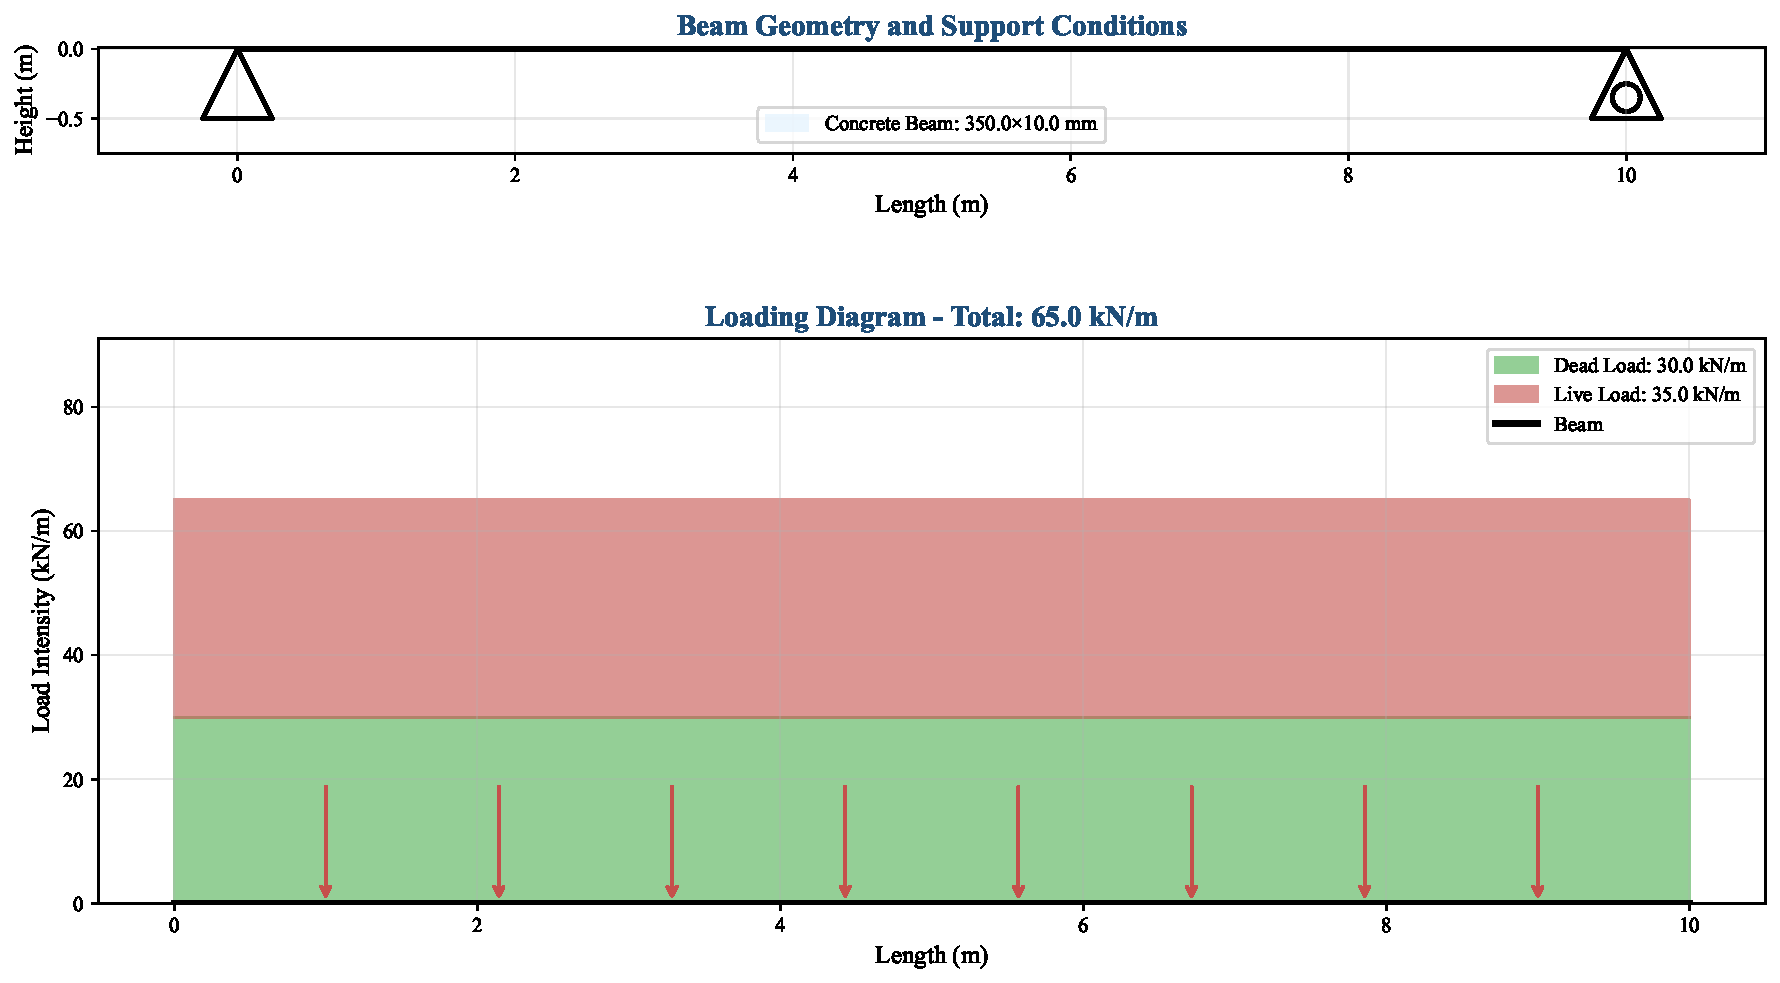
\includegraphics[width=0.9\textwidth]{beam_diagram.pdf}
\caption{Beam geometry, support conditions, and loading configuration}
\label{fig:beam_geometry}
\end{figure}

\begin{figure}[H]
\centering
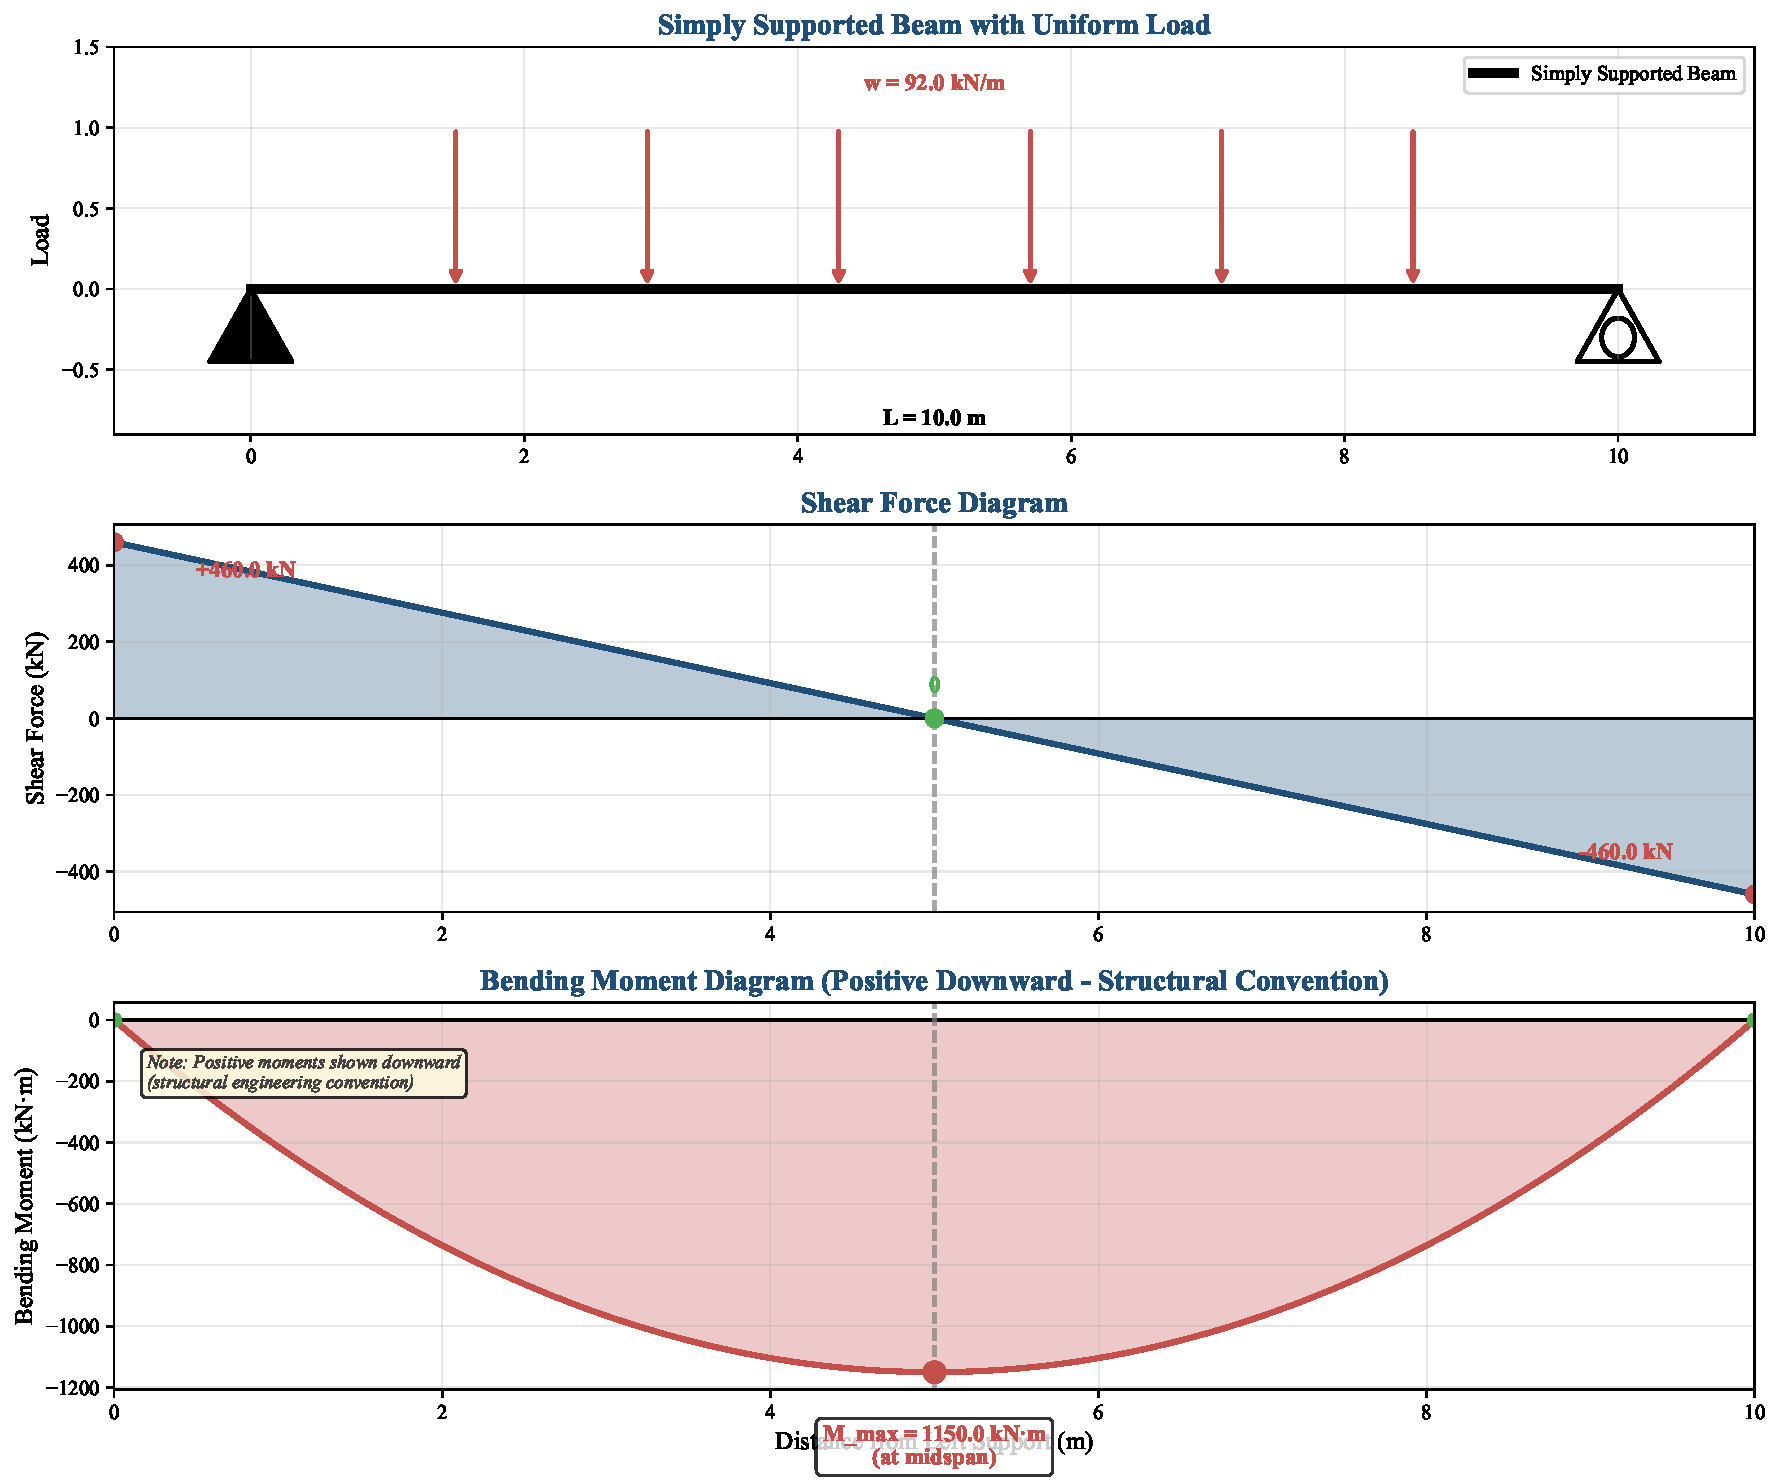
\includegraphics[width=0.9\textwidth]{bmd_sfd.pdf}
\caption{Bending moment and shear force diagrams (positive moments downward)}
\label{fig:bmd_sfd}
\end{figure}

\begin{figure}[H]
\centering
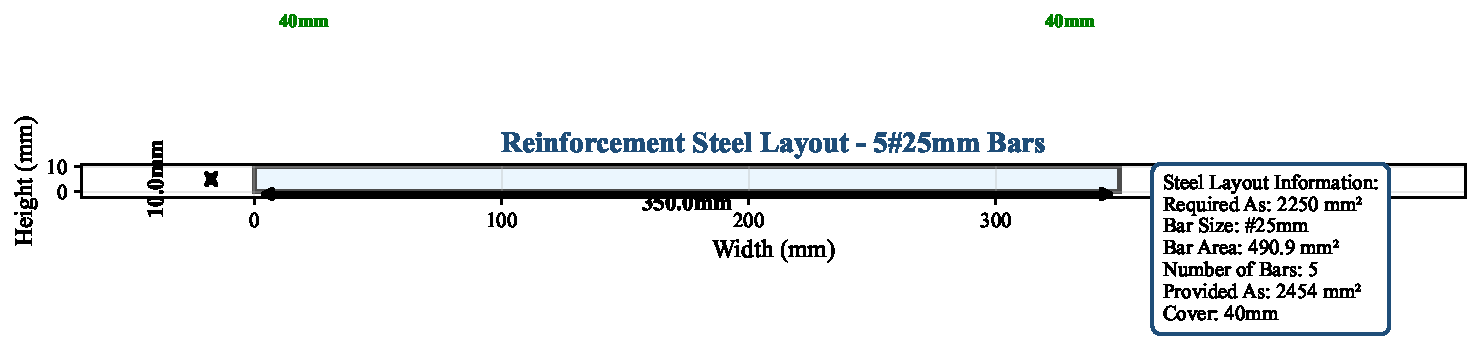
\includegraphics[width=0.8\textwidth]{steel_layout.pdf}
\caption{Reinforcement steel arrangement and detailing}
\label{fig:steel_layout}
\end{figure}

\section{Flexural Design}

\subsection{Required Flexural Reinforcement}

The required area of tensile reinforcement is determined using the strength design method per ACI 318-19 Section 22.2:

\begin{align}
A_{s,req} &= \frac{M_u}{\phi f_y (d - a/2)} = \text{STEEL_AREA_PLACEHOLDER mm}^2 \label{eq:steel_req}
\end{align}

\subsection{Minimum Reinforcement Requirements}

Per ACI 318-19 Section 9.6.1.2, the minimum area of flexural reinforcement shall not be less than:

\begin{align}
A_{s,min} &= \max\left(\frac{0.25\sqrt{f'_c}}{f_y}bd, \frac{1.4}{f_y}bd\right) = \text{MIN_STEEL_PLACEHOLDER mm}^2 \label{eq:steel_min}
\end{align}

\section{Shear Design}

\subsection{Concrete Shear Capacity}

The nominal shear strength provided by concrete is calculated per ACI 318-19 Section 22.5.5:

\begin{align}
V_c &= 0.17\sqrt{f'_c} \, b_w d = \text{CONCRETE_SHEAR_PLACEHOLDER kN} \label{eq:concrete_shear}\\
\phi V_c &= 0.75 \times V_c = \text{PHI_CONCRETE_SHEAR_PLACEHOLDER kN} \label{eq:phi_concrete_shear}
\end{align}

where $\phi = 0.75$ is the strength reduction factor for shear.

\section{Design Verification and Summary}

\subsection{Design Check Summary}

\begin{center}
\renewcommand{\arraystretch}{1.4}
\begin{tabular}{l c c c}
\toprule
\textbf{Design Requirement} & \textbf{Required} & \textbf{Provided} & \textbf{Status} \\
\midrule
Flexural Capacity & REQUIRED_MOMENT_PLACEHOLDER & PROVIDED_MOMENT_PLACEHOLDER & \textcolor{ghaligreen}{\textbf{OK}} \\
Shear Capacity & REQUIRED_SHEAR_PLACEHOLDER & PROVIDED_SHEAR_PLACEHOLDER & \textcolor{ghaligreen}{\textbf{OK}} \\
Minimum Steel Ratio & MIN_RATIO_PLACEHOLDER & PROVIDED_RATIO_PLACEHOLDER & \textcolor{ghaligreen}{\textbf{OK}} \\
\bottomrule
\end{tabular}
\end{center}

\subsection{Design Status}

\textbf{\textcolor{ghaligreen}{DESIGN SATISFACTORY}} - All structural requirements per ACI 318-19 have been satisfied.

\section{Conclusion}

The reinforced concrete beam design has been completed in accordance with ACI 318-19 Building Code Requirements for Structural Concrete. All capacity checks demonstrate adequate structural performance with appropriate safety factors. The design is suitable for construction and meets all applicable code requirements.

\textbf{Key Design Features:}
\begin{itemize}
\item BMD presentation with structural engineering convention (positive downward)
\item High-resolution vector graphics for professional presentation
\item Complete ACI 318-19 compliance verification
\item Professional engineering calculation format
\end{itemize}

\vspace{1.5cm}

% Professional Signature Block
\begin{center}
\renewcommand{\arraystretch}{1.8}
\begin{tabular}{c c}
\toprule
\textbf{Prepared By} & \textbf{Reviewed By} \\
\midrule
& \\
ENGINEER_NAME_PLACEHOLDER & REVIEWER_NAME_PLACEHOLDER \\
Professional Engineer & Professional Engineer \\
Date: \today & Date: \_\_\_\_\_\_\_\_\_\_\_\_\_ \\
\bottomrule
\end{tabular}
\end{center}

\vspace{0.5cm}

\begin{center}
\small\textcolor{ghaligray}{
This calculation has been prepared in accordance with applicable engineering standards and professional practice. \\
All calculations and results are subject to independent review and verification.
}
\end{center}

\end{document} 